\documentclass[dvipsnames,tikz]{standalone}
\usepackage{amsmath}
\usepackage{xcolor}
\usepackage{tikz}
\usetikzlibrary{calc}
\usetikzlibrary{decorations.pathreplacing,calligraphy,3d}


\begin{document}
	% add color=white for dark mode
	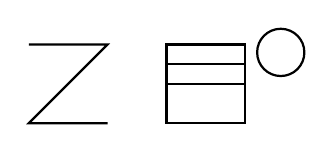
\begin{tikzpicture}[node distance={15mm}, thick, main/.style = {draw}] 
		\begin{scope}
			\path[shape=coordinate]	
			(1,0) coordinate(A) 
			(0,0) coordinate(B) 
			(1,1) coordinate(C) 
			(0,1) coordinate(D);
			
			\draw (A) -- (B) -- (C) -- (D);
		\end{scope}
		
		\begin{scope}[xshift=1.75cm]
			\path[shape=coordinate]	
			(0,0) coordinate(A) 
			(1,0) coordinate(B) 
			(1,1) coordinate(C) 
			(0,1) coordinate(D)
			(1,0.5) coordinate(E)
			(0,0.5) coordinate(F)
			(1,0.75) coordinate(G)
			(0,0.75) coordinate(H);
			
			\draw (A) -- (B) -- (C) -- (D) --cycle;
			\draw (E) -- (F);
			\draw (G) -- (H);
		\end{scope}
		
		\begin{scope}[xshift=3.2cm]
			\draw (0,0.9) circle (0.3);
		\end{scope}
	\end{tikzpicture} 
	
\end{document}